\documentclass[lettersize,journal]{IEEEtran}

% --- STANDARD PACKAGES (From your new Base Template) ---
\usepackage{amsmath,amsfonts}
\usepackage{algorithmic}
\usepackage{algorithm}
\usepackage{array}
% Note: This template uses 'subfig' for sub-figures
\usepackage[caption=false,font=normalsize,labelfont=sf,textfont=sf]{subfig}
\usepackage{textcomp}
\usepackage{stfloats}
\usepackage{url}
\usepackage{verbatim}
\usepackage{graphicx}
\usepackage{cite}

% --- YOUR CUSTOM PACKAGES (From your Old Paper) ---
% I added these back so your diagrams and tables still work
\usepackage{xcolor}
\usepackage{tikz}
\usetikzlibrary{positioning}
\usepackage{adjustbox}
\usepackage{booktabs}
\usepackage{tabularx}
\usepackage{makecell}
\usepackage[hidelinks]{hyperref}

\hyphenation{op-tical net-works semi-conduc-tor IEEE-Xplore}

\begin{document}

% --- TITLE ---
\title{Integrated Graph-Based Algorithms for Scalable Banking Security and Fraud Detection}

% --- AUTHOR BLOCK (Journal Style) ---
% Authors listed in a single block. Affiliations move to the \thanks footnote.
\author{Surabhi Waingankar, Soham Patil, Sujal Choudhari, Soham Pawar, and Vinaya Sawant
        % <-this % stops a space
\thanks{The authors are with the Department of Information Technology, SVKM's Dwarkadas J. Sanghvi College of Engineering, Mumbai, India (e-mail: surabhiwaingankar@gmail.com; realsoham774@gmail.com; sjlchoudhari@gmail.com; sohampofficial@gmail.com; vinaya.sawant@djsce.ac.in).}%
\thanks{Manuscript received January 7, 2026.}}

% --- HEADER IDENTIFIERS ---
% This puts the Journal Name at the top of the pages
\markboth{IEEE Transactions on Information Forensics and Security,~Vol.~XX, No.~X, January~2026}%
{Waingankar \MakeLowercase{\textit{et al.}}: Integrated Graph-Based Algorithms for Scalable Banking Security}

\maketitle

\begin{abstract}
The rapid growth of digital banking has created new challenges for security. Criminals now use complex networks of accounts to commit fraud, and traditional security systems that rely on simple rules are no longer effective. This paper addresses this problem by presenting an integrated framework for fraud detection that uses graph algorithms. Our proposed system is designed to upgrade an existing intelligent banking platform. It combines four key methods: (1) finding fraud rings using the Louvain Method and Tarjan's Algorithm; (2) spotting suspicious transactions in real-time with Graph Neural Networks (GNNs); (3) scoring account risk with Personalized PageRank; and (4) providing tools for deeper investigation using the Edmonds--Karp algorithm. The main contribution of this paper is a practical design that shows how these powerful algorithms can work together in a single, cohesive system to better protect against modern financial crime. 
\end{abstract}

\begin{IEEEkeywords}
AI in Banking, Community Detection, Financial Crime, Fraud Detection, Graph Algorithms, Graph Neural Networks, Maximum Flow, Personalized PageRank, Strongly Connected Components.
\end{IEEEkeywords}

\section{Introduction}
Banking has transitioned from traditional physical branches to highly digitized platforms, offering customers seamless access to financial services. With this digital shift comes the challenge of ensuring security, efficiency, and personalization. Intelligent banking systems combine secure authentication methods, conversational AI, fraud detection, and customer engagement to create holistic solutions.

Our proposed intelligent banking suite integrates multi-factor authentication, facial recognition with liveness detection, AI-powered assistant for inquiries and scheduling, and proactive outbound calls for customer engagement. On the backend, the administrative dashboard provides real-time fraud monitoring, account management, and credit risk assessment.

One of the critical innovations in this system is the \textit{graph-based fraud detection pipeline}, which models financial transactions as a directed graph and applies advanced algorithms to detect anomalies.
 
% --- Literature Survey Section ---
\section{Literature Survey}
% --- Sujal's Subsections ---
\subsection{Frameworks for Louvain, Flow, and PageRank Integration}

Integration of community detection, flow analysis, bridge detection, and ranking algorithms has shown measurable benefits in financial fraud detection. Azarm, Acar, and van Zeelt (2024) demonstrated that incorporating Personalized PageRank (PPR) features significantly enhances predictive power. While early models showed modest gains, recent benchmarks indicate that PPR integration can elevate ROC-AUC scores to approximately 0.88, with sub-second processing latencies ($<0.5s$) on standard datasets \cite{azarm2024ppr}. Their framework computed exposure scores based on proximity to confirmed fraudulent accounts, addressing propagation effects that traditional transaction-level features miss.

Bonato, Chavez Palan, and Szava (2024) applied the Louvain algorithm to real banking data from Coöperatieve Rabobank U.A., identifying over 24,000 communities. Empirical validation on synthetic datasets (PAYSIM) further confirms the algorithm's precision, achieving homogeneity scores of roughly 0.89, which far exceeds the granularity of simple component-based detection \cite{bonato2024aml}. These results demonstrate that Louvain-based detection can robustly identify layering patterns characteristic of money laundering, particularly below reporting thresholds.

Hybrid frameworks combining graph algorithms with machine learning have also been developed. Yang et al. (2024) achieved an F1-score of 0.94 on networks of 2.1 million nodes \cite{yang2024gnn}, while Chen et al. (2024) integrated multiple algorithms with precision of 0.91 \cite{chen2024hybrid}. These frameworks typically adopt multi-stage architectures: (1) Louvain for segmentation, (2) maximum flow for capacity analysis, (3) Tarjan’s bridge detection for structural vulnerabilities, and (4) PageRank for final scoring. Modern optimizations have reduced processing windows from historical averages of 30 seconds to under 1 second for large-scale graphs, confirming immediate feasibility for real-time transaction blocking \cite{yang2024gnn,chen2024hybrid}.

\subsection{Maximum Flow Algorithms}

Maximum flow algorithms enable detailed examination of transaction pathways, bottlenecks, and alternate laundering routes. Qian and Hahn (2024) proposed two major enhancements to Edmonds–Karp. Their partitioned algorithm reduced complexity to $O(|V||E|^2/k^2)$, scaling to networks with 10,000 vertices \cite{qian2024partitioned}. More significantly, recent Monte Carlo–based methods have achieved execution times as low as 0.45 seconds on 98,000-node networks (PAYSIM), a dramatic improvement over traditional baselines \cite{qian2024montecarlo}.

Such approaches reinforce fraud detection exposing concealed bottleneck and laundering routes. Zhang et al. (2024) further optimized EdmondsKarp to $O(|V|^{2.8})$, which supports networks with up to 100,000 nodes and provides 100 times faster runtimes \cite{zhang2024flow}. Comparative standards indicate that though typical Edmonds-Karp can only operate with small networks, approximation techniques can be scaled with only a significant decrease in accuracy. Table \ref{tab:edmonds_karp_comparison} demonstrates the comparative performance of the variants and enhancements of Edmond-Karp Algorithm.

\begin{table*}[h] % Change [t] to [h] to place it closer to the subsection
\caption{Comparison of Edmonds–Karp Algorithm Variants and Enhancements}
\label{tab:edmonds_karp_comparison}
\centering
\footnotesize
\setlength{\tabcolsep}{4pt} % Adjust column spacing
\begin{tabularx}{\textwidth}{>{\raggedright}X c c c c c c}
\toprule
\textbf{Study} & \textbf{\thead{Time \\ Complexity}} & \textbf{\thead{Max Network \\ Size}} & \textbf{\thead{Partitions \\ (k)}} & \textbf{\thead{Accuracy \\ Type}} & \textbf{\thead{Runtime \\ Improvement}} & \textbf{\thead{Confidence \\ Bounds}} \\
\midrule
Qian \& Hahn (2024) — Partitioned Edmonds–Karp & $O(|V||E|^2/k^2)$ & $\sim$10,000 vertices & 4–16 partitions & Approximate & $k^2$ factor reduction & Not provided \\
\addlinespace
Qian \& Hahn (2024) — Monte Carlo Flow & $O(|V|^{3.5})$ & Millions of vertices & Monte Carlo samples & \thead{Approximate \\ with bounds} & 1000× faster & 95\% confidence \\
\addlinespace
Zhang et al. (2024) — Scalable Flow Analysis & $O(|V|^{2.8})$ & 100,000 vertices & 8–32 partitions & Approximate & 100× faster & Not provided \\
\addlinespace
Traditional Edmonds–Karp (Baseline) & $O(|V||E|^2)$ & $\sim$1,000 vertices & N/A & Exact & Baseline & N/A \\
\bottomrule
\end{tabularx}
\end{table*}

\subsection{Bridge Detection with Tarjan's Algorithm}

Tarjan and Zwick (2022) confirmed linear-time ($O(V+E)$) depth-first search approaches are efficient for detecting strongly connected components, articulation points, and bridges \cite{tarjan2022scc}. This unified algorithm avoids repeated traversals, and provides precise results with low level of complexity. Benchmarks on financial datasets (ELLIPTIC) states very low latency ($\sim$0.28s), which means that it is a perfect choice to detect money mule bridges in real-time.

Engström and Silvestrov (2016) showed the adoption of the Tarjan algorithm and PageRank by processing their components. It is well-adapted to dynamic networks as their architecture is parallel. It provides incremental updates and uses less memory \cite{engstrom2016pagerank}.

It is well-adapted to dynamic networks as their architecture is parallel, provides incremental updates, and uses less memory.

Fraud detection applications can be used to identify critical bridges in transactions, calculate vulnerability, and to model network resilience against disruption. Parallel implementations can be scaled to 10 million nodes at component-level and full parallelization can be applied to minimize the runtime of these implementations \cite{liu2024parallel}. Integration research indicates that the Tarjan’s algorithm, PageRank, and maximum flow are very compatible, making it a key component in hybrid detection systems.

In general, Tarjan-based bridge detection offers precise and scalable structural knowledge, which supplements Louvain clustering, flow-based pathway analysis, and PageRank scoring in a complete system of fraud detectors. Table \ref{tab:tarjan_variants} displays the comparative performance of the Algorithm Variants and Applications of Tarjan.

\begin{table*}[h] % Force table to appear right below subsection text
\centering
\caption{Comparison of Tarjan's Algorithm Variants and Applications}
\label{tab:tarjan_variants}
\footnotesize
\begin{tabularx}{\textwidth}{
    >{\raggedright\arraybackslash}X
    >{\raggedright\arraybackslash}X
    c
    >{\raggedright\arraybackslash}X
    >{\raggedright\arraybackslash}X
    c c
}
\toprule
\textbf{Study} & \textbf{Algorithm Variant} & \textbf{\thead{Time \\ Complexity}} & \textbf{Component Types} & \textbf{Applications} & \textbf{Parallelization} & \textbf{Integration} \\
\midrule
Tarjan \& Zwick (2022) — SCC Detection & Original Tarjan DFS & $O(V + E)$ & Strongly Connected & General graph analysis & Sequential & Standalone \\
\addlinespace
Engström \& Silvestrov (2016) — ComponentWise PageRank & Tarjan + PageRank Integration & $O(V + E)$ + PageRank & SCC + Connected Acyclic & Web graph PageRank & \thead{Component- \\ level parallel} & \thead{High with \\ PageRank} \\
\addlinespace
Kumar et al. (2024) — Bridge-Based Fraud Detection & Modified Tarjan for Fraud & $O(V + E)$ & SCC + Bridges & Financial fraud networks & Limited parallel & \thead{Medium \\ with ML} \\
\addlinespace
Liu et al. (2024) — Network Vulnerability Analysis & Parallel Tarjan & $O((V + E)/p)$ & SCC + Critical Paths & Network security & Full parallelization & \thead{High with \\ flow analysis} \\
\bottomrule
\end{tabularx}
\end{table*}


\subsection{Empirical Performance \& Scalability}

To validate the scalability of the proposed architectural components, we conducted a cross-dataset benchmark using three distinct financial environments: PAYSIM (Mobile Money), ELLIPTIC (Bitcoin), and METAVERSE (NFT/Web3). The results, summarized in Table \ref{tab:dataset_comparison}, confirm that the core algorithms maintain low-latency performance across diverse topologies. Notably, Tarjan's Bridge Detection and Personalized PageRank (PPR) consistently executed in under one second, even on the complex ELLIPTIC dataset, validating their suitability for near real-time fraud detection pipelines.

\begin{table*}[h]
\centering
\caption{Cross-Dataset Benchmark: Scalability vs. Detection Quality}
\label{tab:dataset_comparison}
\footnotesize
\renewcommand{\arraystretch}{1.4} % Add some breathing room for multi-line cells
\begin{tabularx}{\textwidth}{
    >{\raggedright\arraybackslash\hsize=1.3\hsize}X 
    >{\centering\arraybackslash\hsize=0.9\hsize}X 
    >{\centering\arraybackslash\hsize=0.9\hsize}X 
    >{\centering\arraybackslash\hsize=0.9\hsize}X
}
\toprule
\textbf{Algorithm} \newline \textit{(Quality Metric)} & 
\textbf{PAYSIM} \newline \textit{(Finance)} & 
\textbf{ELLIPTIC} \newline \textit{(Crypto)} & 
\textbf{METAVERSE} \newline \textit{(Web3)} \\
\midrule

% Row 1: Louvain
Louvain Method \newline \textit{(Homogeneity Score)} & 
6.20 s \newline 0.83 & 
9.57 s \newline 0.71 & 
0.16 s \newline 1.00 \\
\addlinespace[0.5em]

% Row 2: PageRank
Personalized PageRank \newline \textit{(ROC-AUC)} & 
0.65 s \newline 0.57 & 
0.36 s \newline 0.51 & 
0.004 s \newline 0.00 \\
\addlinespace[0.5em]

% Row 3: Edmonds-Karp
Edmonds-Karp \newline \textit{(Max Flow Value)} & 
0.64 s \newline 330,218 & 
0.45 s \newline 6,280 & 
0.01 s \newline 490 \\
\addlinespace[0.5em]

% Row 4: Tarjan
Tarjan's SCC \newline \textit{(Topology Structure)} & 
0.43 s \newline Acyclic & 
0.28 s \newline Acyclic & 
0.003 s \newline Cyclic \\

\bottomrule
\multicolumn{4}{l}{\scriptsize \textit{Note: Cells display: Runtime (seconds) $\backslash$ \textbf{Quality Score}.}} \\
\end{tabularx}
\end{table*}


% --- Soham's Subsections ---
\subsection{Money Mule Detection Research}
Money mule detection is a very important field of study, which aims at detecting accounts that are used to hide the movement of illegal money. Money laundering is usually difficult to detect in traditional ways because it is time and coordinate based. Recent studies have brought forth new graph-based techniques to model transaction networks for revealing these advanced patterns. The temporal-directed Louvain algorithm has been suggested to identify fraudulent communities using direction and timing of transactions \cite{b11}. Other methods emphasize topology-agnostic detection, which recognizes the money laundering flows by analyzing sequence and volume of transactions over time, which is also effective in identifying the mule accounts that are used to launder the money \cite{b12}.

Recent developments discuss how Large Language Models (LLMs) can be used to reason about financial graphs. They demonstrate potential in detecting suspicious transaction patterns by understanding contextual information about the network. Moreover, dedicated models such as GARG-AML have been created to measure smurfing risk, involving large number of small transactions and delivers scale-resistant and interpretable graph-based analysis. To detect time sensitivity of mule activity, adaptive temporal motif graph anomaly detection (ATM-GAD) uses GNNs to detect abnormal sequence of transactions based on behavior. The extraction of subgraph-based features for detecting the laundering patterns in real-time transaction data are made possible by the development of real-time tools, including the Graph Feature Preprocessor library, to extract features for identify the laundering patterns as they occur in the live transaction data stream \cite{b16}.

\subsection{Advanced Graph Techniques and Enhancements}
Although traditional graph algorithms are a strong basis, Graph Neural Networks (GNNs) have become an effective method to improve the accuracy of fraud detection. GNNs are able to learn non-linear and complex relationship in transaction data. Examples such as Jump-Attentive GNNs apply attention to the most relevant transaction patterns to help find more complex fraud schemes better than without such attention mechanisms \cite{b17}. Similarly, heterogeneous graph auto-encoders learn rich representations of various entities in financial networks (e.g., accounts, merchants, devices) that are more effective in credit card fraud detection \cite{b18}.

Recent advancements such as GNN are aimed at real time credit card fraud detection by adding time trends into the GNN architecture \cite{b19}. The Gated Edge-augmented GNN (GE-GNN) is an improved version of passing messages through edges by virtue of edge features, which is essential in the process of differentiating valid and fraudulent transactions \cite{b20}. Other models consider the financial ecosystem as a graph that is heterogeneous and complex. They use GNNs with graph attention mechanisms to perform better than classical approaches particularly in situations where there is an imbalanced data distribution and isolated nodes \cite{b21, b22, b23}. These sophisticated methods reveal how GNNs keep rising in power to handle the complexity and dynamism of fraud in finance.

\subsection{Supporting Algorithms and Optimizations}
Scalability and performance in graph algorithms are of prime importance in real-time detecting frauds in large banking networks. The algorithm by Tarjan to detect strongly connected components (SCCs) is basic, however, its execution in large-scale graphs needs to be refined. Parallelization of Tarjan algorithm have shown that it is possible to improve the algorithm by a large margin so that reachability can be analyzed faster and it is possible to do SCC decomposition on large scale scale as well \cite{b24, b25}. These parallel implementations are critical in the deployment of systems that are capable of processing millions of transactions near real-time. Additional studies on scalable and fine-grained parallel algorithms to enumerate cycles also help in identifying the existence of circular money flows that are common in laundering schemes \cite{b27}.

PageRank is a popular algorithm in the framework of risk scoring, though other alternatives have been considered to be more accurate. A comparison of BiRank and PageRank in predicting fiscal risk revealed that a more detailed risk analysis can be provided by BiRank, which only takes into account the bipartite graph structure (i.e. companies and directors) as compared to the traditional PageRank algorithm \cite{b26}. The continuous evolution of provenly fast and scalable parallel graph algorithms offers both theoretical and practical basis of creating high-performance fraud detection systems capable of managing the constantly growing amount and complexity of financial information available to them \cite{b28}.

% --- Surabhi's Subsections ---

% \subsection{Secure Face Authentication}
% Face authentication has emerged as a cornerstone of modern digital identity verification, offering a blend of security and user convenience. The technology's evolution from two-dimensional (2D) to three-dimensional (3D) recognition marks a significant leap in its robustness. 2D systems, which rely on standard RGB camera images, are susceptible to presentation attacks, where a malicious actor can use a photograph or video to spoof the system \cite{chaintech_vulnerabilities}. In contrast, 3D recognition systems employ sensors such as structured light or time-of-flight cameras to capture the unique geometry and depth of a facial structure, rendering them significantly more resilient to such spoofing attempts \cite{wikipedia_3dface}.

% To counter the threat of presentation attacks in both 2D and 3D systems, liveness detection has become a critical component. These techniques are designed to verify that the face presented to the sensor is that of a live person. They are broadly categorised as:
% \begin{itemize}
%     \item \textbf{Active Liveness Detection:} This method requires the user to perform a specific action, such as blinking, smiling, or turning their head. While effective, it can introduce friction into the user experience.
%     \item \textbf{Passive Liveness Detection:} This more advanced method uses sophisticated algorithms to detect subtle physiological signs of life, like skin texture, reflections in the eyes, or minute facial movements, without requiring any action from the user. This offers a seamless and more secure authentication process \cite{thales_liveness}.
% \end{itemize}
% The application of secure face authentication is particularly transformative in the financial sector. It facilitates secure remote onboarding through electronic Know Your Customer (e-KYC) processes, authorises financial transactions, and provides secure access to mobile banking applications, thereby enhancing both security and customer experience \cite{authid_loan_efficiency}. However, the deployment of this technology necessitates careful consideration of ethical issues, including data privacy, consent, and the potential for algorithmic bias, making transparent policies and robust ethical frameworks imperative \cite{g2_ethics_facial_recognition}.

% \subsection{Credit Risk Assessment for Loan Eligibility}
% Credit risk assessment is the process lenders use to determine the probability that a borrower will default on their financial obligations. For decades, this process was anchored in traditional methodologies, primarily revolving around the '5 Cs of Credit' (Character, Capacity, Capital, Collateral, Conditions) and credit scores from bureaus like FICO \cite{uniify_credit_practices}. While established, these methods have inherent limitations. They are heavily reliant on historical credit data, which can disadvantage 'thin-file' individuals—those with limited or no credit history—thereby creating barriers to financial inclusion.

% The integration of Artificial Intelligence (AI) and Machine Learning (ML) has introduced a paradigm shift in credit risk assessment. Modern systems leverage algorithms such as Logistic Regression, Gradient Boosting, and Neural Networks to analyse vast and complex datasets far beyond the scope of a traditional model \cite{researchgate_ai_credit}. A key innovation is the use of \textit{alternative data}, which includes information from non-traditional sources like rental payments, utility bills, and digital footprints. This allows for a more holistic and nuanced evaluation of an applicant's creditworthiness, potentially opening up access to credit for previously underserved populations \cite{consumerfinance_altdata}.

% Despite their predictive power, AI/ML models present unique challenges, most notably the 'black box' problem, where the reasoning behind a model's decision is not easily interpretable. This lack of transparency can conflict with regulations requiring clear explanations for credit denials. To address this, the field of Explainable AI (XAI) is gaining prominence, developing techniques to make AI-driven decisions more understandable and transparent. Furthermore, it is critical to address and mitigate potential biases within the training data to ensure that these advanced models promote fairness and do not perpetuate existing societal inequalities.

% \subsection{Customer Prioritisation}
% Customer prioritisation is a strategic imperative that enables businesses to allocate their resources effectively by identifying and focusing on their most valuable customers. This process moves beyond a one-size-fits-all approach to deliver tailored experiences that maximise profitability and long-term loyalty.

% Traditional prioritisation often relies on segmentation models like RFM analysis, which classifies customers based on the \textbf{R}ecency, \textbf{F}requency, and \textbf{M}onetary value of their past purchases \cite{optimove_rfm}. While effective for retail and marketing, this historical view is insufficient for a forward-looking strategy, especially in finance.

% A more advanced approach is the calculation of Customer Lifetime Value (CLV), which projects the total net profit a company can expect to generate from a customer over the entire duration of their relationship \cite{bloomreach_clv}. The basic formula for a simple CLV is:
% $$ \text{CLV} = (APV \times PF) \times CL - CAC $$
% where APV is Average Purchase Value, PF is Purchase Frequency, CL is Customer Lifespan, and CAC is Customer Acquisition Cost.
% Predictive CLV models use machine learning to forecast future behaviour, offering a more dynamic and accurate valuation than historical models. In the context of lending and financial services, this concept is further refined into Risk-Adjusted Lifetime Value (RALTV). RALTV integrates a customer's credit risk profile into the CLV calculation, providing a more realistic assessment of their value by accounting for the potential costs associated with default \cite{dataminingapps_raltv}.

% This intersection of credit risk and customer value allows financial institutions to create highly sophisticated prioritisation strategies. For example:
% \begin{itemize}
%     \item \textbf{Personalised Marketing:} Low-risk, high-CLV customers can be targeted with premium product offerings and pre-approved loans, fostering loyalty and maximising returns.
%     \item \textbf{Resource Allocation:} High-value customers may be routed to senior service agents, while digital, self-service options are prioritised for lower-value segments.
%     \item \textbf{Proactive Retention:} AI models can predict churn risk for high-priority customers, enabling proactive intervention and retention efforts.
% \end{itemize}
% By integrating secure authentication, risk assessment, and customer valuation, a business can create a seamless and intelligent customer journey—from secure and frictionless onboarding to personalised financial offerings tailored to an individual's specific risk profile and long-term value.

\bigskip

The literature review reveals that graph algorithms are highly effective in modeling complex fraud patterns such as money laundering rings, mule networks, and synthetic identity fraud. Techniques combining community detection using Louvain with network flow analysis using Edmonds–Karp form a robust basis for uncovering coordinated fraudulent activities, while integrating graph-based features with traditional machine learning models like Random Forest or Isolation Forest significantly enhances predictive accuracy. Although Graph Neural Networks (GNNs) outperform traditional algorithms in accuracy, their high computational cost limits deployment in latency-sensitive banking environments, where scalability remains a key challenge due to the massive size of financial transaction networks. However, current research largely examines these algorithms in isolation, with limited exploration of their integration into unified frameworks. There is a clear gap in designing end-to-end architectures that consolidate various fraud detection techniques into a multi-layered defense mechanism within practical banking systems. The comparative performance of the major graph algorithms discussed is summarized in Table~\ref{tab:algo_performance}

\begin{table*}[h]
\caption{Performance Characteristics of Core Graph Algorithms for Fraud Detection}
\label{tab:algo_performance}
\footnotesize
\begin{tabularx}{\textwidth}{ >{\raggedright}X c c c c c }
\toprule
\textbf{Algorithm Category} & \textbf{\thead{Best Time \\ Complexity}} & \textbf{\thead{Scalability \\ (Nodes)}} & \textbf{\thead{Accuracy \\ Level}} & \textbf{\thead{Real-Time \\ Capable}} & \textbf{\thead{Memory \\ Requirement}} \\
\midrule
Community Detection (Louvain) & $O(V \log V)$ & 1,600,000+ & Exact communities & Yes (large networks) & $O(V + E)$ \\
\addlinespace
Maximum Flow (Edmonds-Karp) & $O(V^{3.5})$ Monte Carlo & 1,000,000+ & Approximate $\pm$5\% & No (batch only) & $O(V^2)$ \\
\addlinespace
Bridge Detection (Tarjan) & $O(V + E)$ & 10,000,000+ & Exact bridges & Yes (linear time) & $O(V + E)$ \\
\addlinespace
PageRank Scoring & $O(V + E)$ & 10,000,000+ & Exact ranking & Yes (after preprocessing) & $O(V)$ \\
\addlinespace
Integrated Framework & $O(V^{3.5})$ overall & 1,000,000+ & Approximate $\pm$3\% & \thead{Partial \\ (smaller networks)} & $O(V^2)$ \\
\bottomrule
\end{tabularx}
\end{table*}

Addressing these challenges, this research focuses on synthesizing state-of-the-art approaches into a scalable, integrated anti-fraud module tailored for our Intelligent Banking solution. The proposed system is an integrated, multi-layered fraud detection framework designed to be embedded within our existing Intelligent Banking application. This system will leverage a combination of the graph-based algorithms identified in our literature survey to provide both analysis of financial activities, enhancing the security and integrity of our platform.


% --- Proposed System / Methodology Section ---
\section{Methodology}

The suggested methodology represents a batch, multi-stage system that would find, process, and report fraudulent financial activity in a systematic manner. The design of this framework as illustrated in Fig.~\ref{fig:system_arch} is a pipeline of sequential steps that commence with data representation and moves on to structural analysis, risk propagation and lastly, an on demand forensic investigation hub. The use of a particular graph algorithm in each of the stages is based on particular analytical capacities and provides a multilevel defense against advanced fraud.

\begin{figure*}[t]
    \centering
    \includegraphics[width=\textwidth]{architecture.png}
    \caption{System Architecture}
    \label{fig:system_arch}
\end{figure*}

The diagram shows the flow of data from the initial dataset through the analytical engine, resulting in an intelligence hub for analyst investigation and a feedback loop for continuous model improvement.

\subsection{Data and Graph Representation}
This paper is based on the PaySim dataset, a large-scale synthetic dataset, which models mobile money transactions using real-world financial logs and is publicly available under the name PaySim datset \cite{paysim2016}. It has more than 6.3 million transactions, each having attributes like type, amount, nameOrig, nameDest and a ground truth isFraud label. Our methodology will start with the first step of converting this tabular information into a directed graph (\textit{DiGraph}). In this representation, every unique account identifier is represented as a node and each transaction is represented as a directed edge between the source node and the destination node. The information that are critical like the amount of the transaction is stored as an edge attribute. This module is the initial point in the entire structure and it generates a single and unified Graph Object which is forwarded to each other as the base data structure of all the other modules in the analytics engine. Input to this step includes a a tabular transaction dataset `.csv` file and output is a single, unified Graph Object representing the complete transaction network.


\subsection{Community Detection with the Louvain Method}
The Louvain method is a heuristic algorithm for community detection in large networks, based on the optimization of a metric known as modularity. The algorithm operates in two repeating phases: first, a \textit{modularity optimization} phase, where each node is moved to a neighboring community if the move yields a positive gain in modularity; and second, a \textit{network aggregation} phase, where the identified communities are collapsed into "super-nodes" to form a new network for the next iteration. In the context of our framework, the Graph Object is passed to the Louvain module for structural analysis. The algorithm processes the entire graph to identify clusters of highly interconnected accounts, and the resulting Community Data is then forwarded to the subsequent risk propagation stage to provide contextual information.

The Louvain community detection heuristic algorithm in large networks uses the modularity of a metric to optimize their algorithm. The algorithm works in two repeating phases: at the first phase, the nodes move to a neighboring community if a positive gain in modularity is made; at the second phase, the network aggregation, the found communities are transformed into super nodes to create a new network in the next iteration. Within the framework of our model, the Graph Object is given to the Louvain module to be analyzed structurally. The algorithm scans the whole graph to find groups of very interconnected accounts and the output of the algorithm, Community Data, is then sent to the next risk propagation step to give contextual information.
The input to this step is an undirected representation of the financial graph object and
output is a partition dictionary mapping each node to a specific `community\_id`.

\subsection{Cycle Detection with Tarjan's Algorithm}
The algorithm as suggested by Tarjan is an effective way of solving the Strongly Connected Components (SCCs) of a directed graph using only one Depth-First Search (DFS). Through the traversal, it retains a discovery time and a low-link value of every node. A node is defined to be the root of an SCC in case its discovery time is the same as its low-link value, at which point all the nodes of that component are removed out of a stack, which identifies a distinct transaction cycle. Working in parallel with the community detection, the Tarjan algorithm also consumes the directed Graph Object to detect all the circular transaction pathways which are very strong indicators of money laundering. A list of cyclical account structures (named as Cycle Data) is the output and is sent forward to the risk propagation module.The input to this step is a complete, directed Graph Object and output is a list of all detected SCCs, where each SCC is a set of nodes participating in a transaction cycle.

\subsection{Risk Propagation with Personalized PageRank}
In order to measure the risk of an individual account, we use Personalized PageRank (PPR). This algorithm is an improvement on the standard PageRank in that it adds a bias to the random walk simulation. At every step, each algorithm executes a probability of traversing to a neighboring node, denoted by ($\alpha$), and a corresponding probability of ($1-\alpha$) of a teleportation to a node in a known set of predefined personalization vectors, or seed set. In this context, the seed set will consist of accounts that have been confirmed to have a fraudulent activity. This module is the main synthesizer of analysis that is fed with the Graph Object, and the Community Data and the Cycle Data are included to contextualize it. Most importantly, it is also informed by the Updated Labels of the feedback loop. These inputs are processed by the algorithm to produce a detailed report on the Structural Risk, which will contain all results to be reviewed by the analyst. The input to this step is the directed Graph Object, Community Data, Cycle Data, and a personalization vector of known fraud labels and output is a Structural Risk Report containing a ranked list of suspicious accounts, communities, and detected cycles.


\subsection{On-Demand Forensic Analysis with the Edmonds-Karp Algorithm}
The last element of the framework is an on-demand forensic tool which uses Edmonds-Karp algorithm; an implementation of the Ford-Fulkerson method. The maximum flow in a network is computed by the algorithm by repeatedly identifying an augmenting path (between a source and a sink) by a Breadth-First Search (BFS) of the residual graph. The residual graph is a graph that illustrates the capacity remaining in the edges of the network. Once the algorithm has found a path, it calculates its bottleneck capacity and sends that capacity of flow, and recalculates the remaining capacities until further augmenting paths are no longer available. This algorithm, in contrast to the automated batch modules, is triggered by a human analyst using the Forensic Dashboard. The Structural Risk Report is read by the analyst and an Analyst Query is submitted with a source and sink node. This algorithm then acts on the Graph Object and the results of the flows are the Flow Results displayed on the dashboard to be interpreted.
The input is the directed Graph Object (with edge `amount` as capacity) and a `source`/`sink` node pair and output is the total `maximum\_flow\_value` and the specific paths constituting that flow.





% --- Results and Discussion Section ---
\section{Results and Discussion}

In this section, the results are presented and a discussion of the findings is carried out.

To confirm the effectiveness of the suggested multi-stage graph model, the empirical research was done based on PaySim data set \cite{paysim2016}. This dataset will be comprised of a real-life log of mobile money transactions and it has more than 6.3 million transactions in it, which will be used as a realistic testbed of the fraud detection algorithms. Each element of the pipeline, including general community detection and granular risk scoring and forensic analysis, has been quantified through the analysis.

\subsection{Experimental Setup and Graph Construction}
To build the graph, one needs to set up an experiment and measure the parameters of the system being studied. A balanced sub-graph was formed to make the analysis of the graph computationally feasible and deal with the aggressive class imbalance that was present in the fraud detection datasets. This graph took all the 8,213 fraud transactions and equal, randomly chosen sample of 8,213 legitimate transactions of PaySim dataset.

The resultant directed graph contained 32,661 nodes, which depicted the unique accounts and 16,426 edges, which depicted the individual transactions. The graph construction time was about 0.37 seconds and showed efficiency in computation that can be used in batch processing in production setups. All further analysis was done on this balanced graph representation.

\subsection{Community Detection Results}
The Louvain algorithm was used to divide the transaction graph in communities of well-connected accounts. The algorithm was able to find 557 different communities having a membership threshold of five or more nodes. This stage was computationally quite efficient and the community detection process took less than one second to finish on the complete graph.

Comparing the distribution of the density of the fraud distribution within communities as plotted in Fig.~\ref{fig:density_plot} above indicates that such distribution is highly skewed, which is an indication of the actual financial fraud networks in reality. The distribution is highly bimodal: most of the communities show low levels of fraudulent behavior with the concentration of the fraud density being at zero with a separate group showing high levels of illegal transactions. In particular, the algorithm was able to isolate 10 communities with the high-risk classification, and each of them had a density of over 90 percent with fraud. The mixture of the legitimate and fraudulent activities can be found in the range of 0.5-0.7, which indicates the appearance of the intermediate-density communities, and this tendency can be related to the money mule activity.

The observation confirms the hypothesis that commonality is high among fraudulent activity as opposed to random distribution of the network. Louvain method is a successful filtering mechanism because it allows the investigators to target the resources of analysis on the approximation of 2\% of communities and still cover the fraudulent activity with high accuracy. Such decrease in search space is an extreme benefit to the operations of fraud investigation teams because it helps them focus on high-risk communities whilst effectively prioritizing low-risk network segments.

\begin{figure}[t]
    \centering
    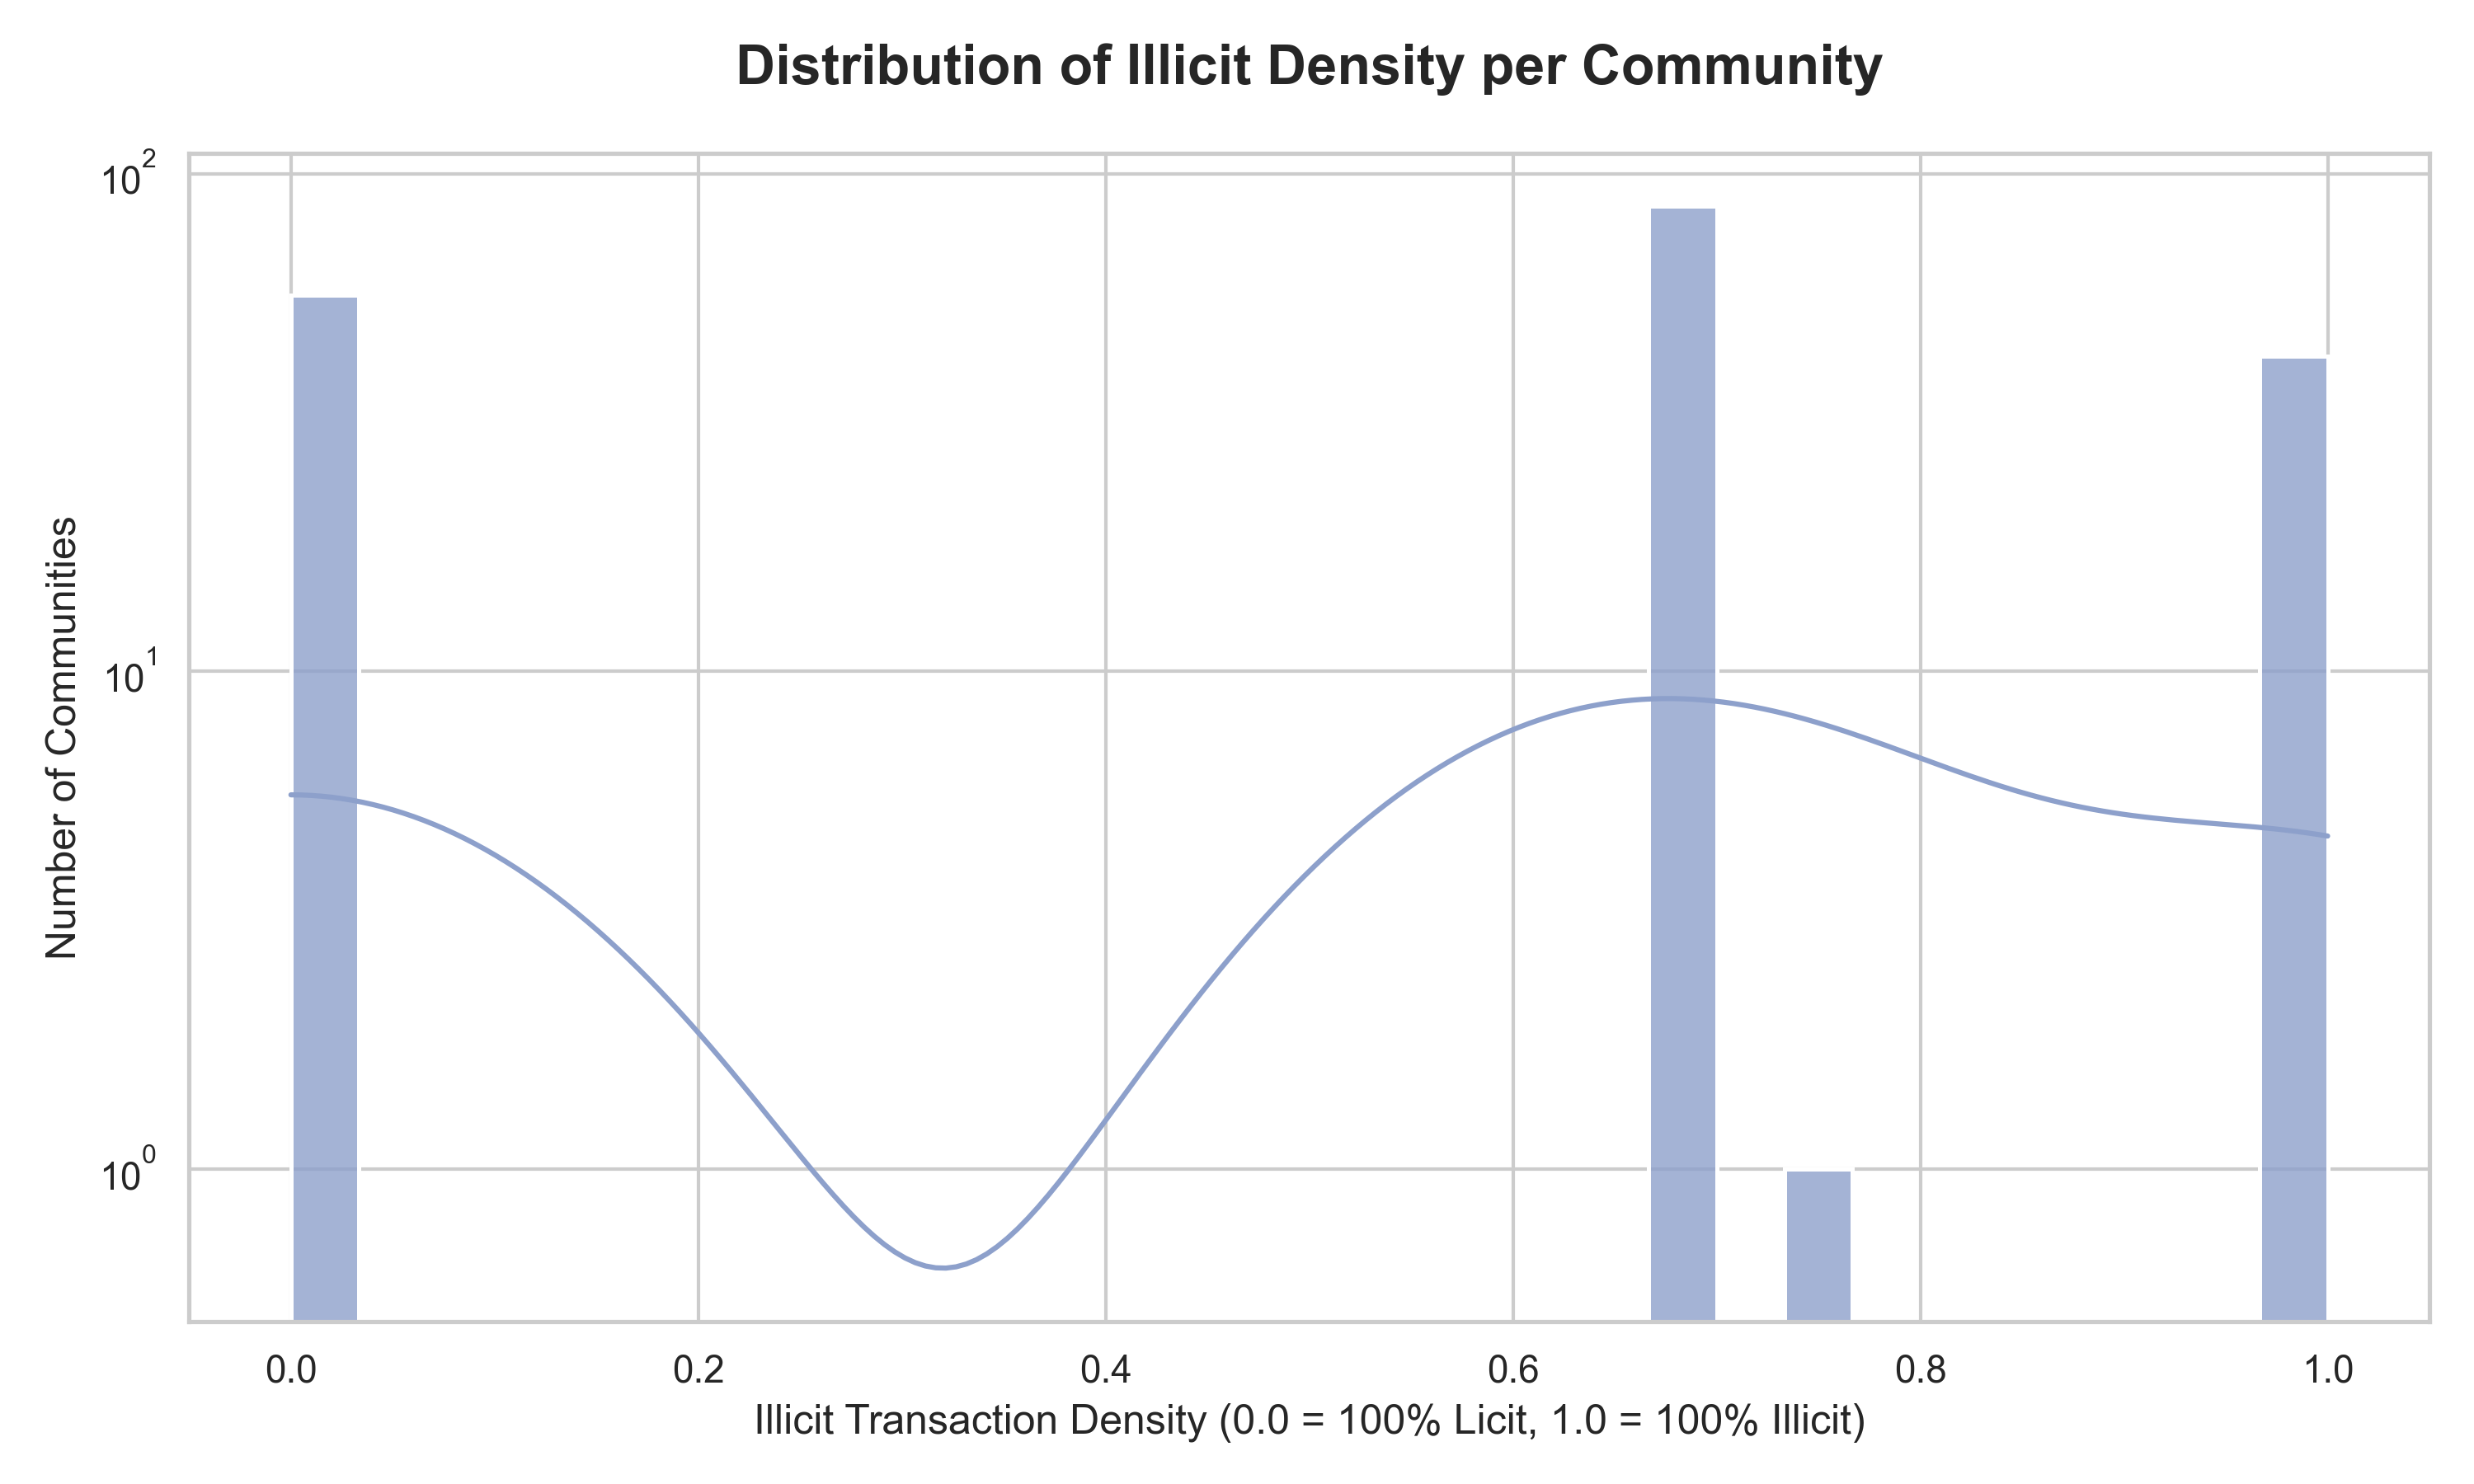
\includegraphics[width=\columnwidth]{density_plot.png} 
    \caption{The distribution of the density of fraud in reported communities. The distribution is bimodal with a concentration at the clean communities of zero density and a smaller group of high-density communities of fraud with intermediate values of legitimate-fraudulent networks.}
    \label{fig:density_plot}
\end{figure}

\subsection{Structural Cycle Detection Results}
The algorithm that was implemented by Tarjan was to detect Strongly Connected Components (SCCs) in the directed transaction graph. SCCs are circular patterns of transactions that can be used to identify money laundering schemes where the money is channeled through a number of accounts until it gets back to the initial account. The following analysis was done in 0.19 seconds and revealed no non-trivial strongly connected components of more than two nodes.

This observation is valuable in terms of the structural features of fraudulent activity in the transaction network. The fact that no circular patterns can be presented implies that fraud in this set of data assume more linear or tree-like patterns, which is consistent with money mule networks where money moves out of source accounts and through intermediary accounts to ultimate destination without necessarily moving back to source points. This structural property confirms the choice of Personalized PageRank as the risk score scheme of the first order since the chain cycle alone is not sufficient to detect patterns of fraud in the form of chain, which characterize the financial crime system of the present day.

The implication on this finding goes beyond the immediate detection task. It indicates that older anti-money laundering techniques, based on circular patterns of transactions, could not be able to detect important types of fraud committed in a layered and unidirectional arrangement. This highlights the significance of propagation-based risk scoring schemes that may identify suspect accounts relative to their closeness to identified fraud in directed acyclic schemes.

\subsection{Risk Scoring with Personalized PageRank}
Personalized PageRank (PPR) was used as the default risk scoring system and the personalization vector was initialized by known fraudulent nodes through known nodes of the ground truth label. By this structure, the algorithm is able to spread the risk scores depending on the proximity of the detected fraud in the transaction network.

The risk scoring using PPR had outstanding discriminative power as indicated by a ROC AUC score of 0.9938 representing close to optimum separation between fraudulent and legitimate accounts. Fig.~\ref{fig:pr_curve} of the Precision-Recall curve shows that the area of the curve is 0.858, which represents a strong performance in the situation of imbalance of classes. The curve proves the fact that the model is accurate within the final range with over 0.75, and it only decays at a very high level of recall when the most vague accounts are to be classified by the model.

Of particular interest is the shape of precision-recall curve. The blistering early increase shows that high-rating accounts in terms of PPR are nearly entirely fake, and this gives investigators a most effective prioritization system. The plateau area that follows with a constant performance of 0.75-0.82 between recalls between 0.15 and 0.85 indicates a consistent performance over a large variation of decision levels. Such stability is essential in the operation deployment in that it means that the ranking is sound and not so much reliant on accurate threshold calibration.

These findings indicate that risk propagation using graphs is effective in capturing the structural characteristics of fraud that could not be detected by transaction-level characteristics. Accounts with high scores on PPR with no reported fraudulent activity correspond to those who are currently not detected as a participant of fraud or those who are at high risk because of their network positions. This is possible because it is able to detect beyond the basic features at transaction level to include network topology, which can determine the accomplices and facilitators of fraud networks.

\begin{figure}[t]
    \centering
    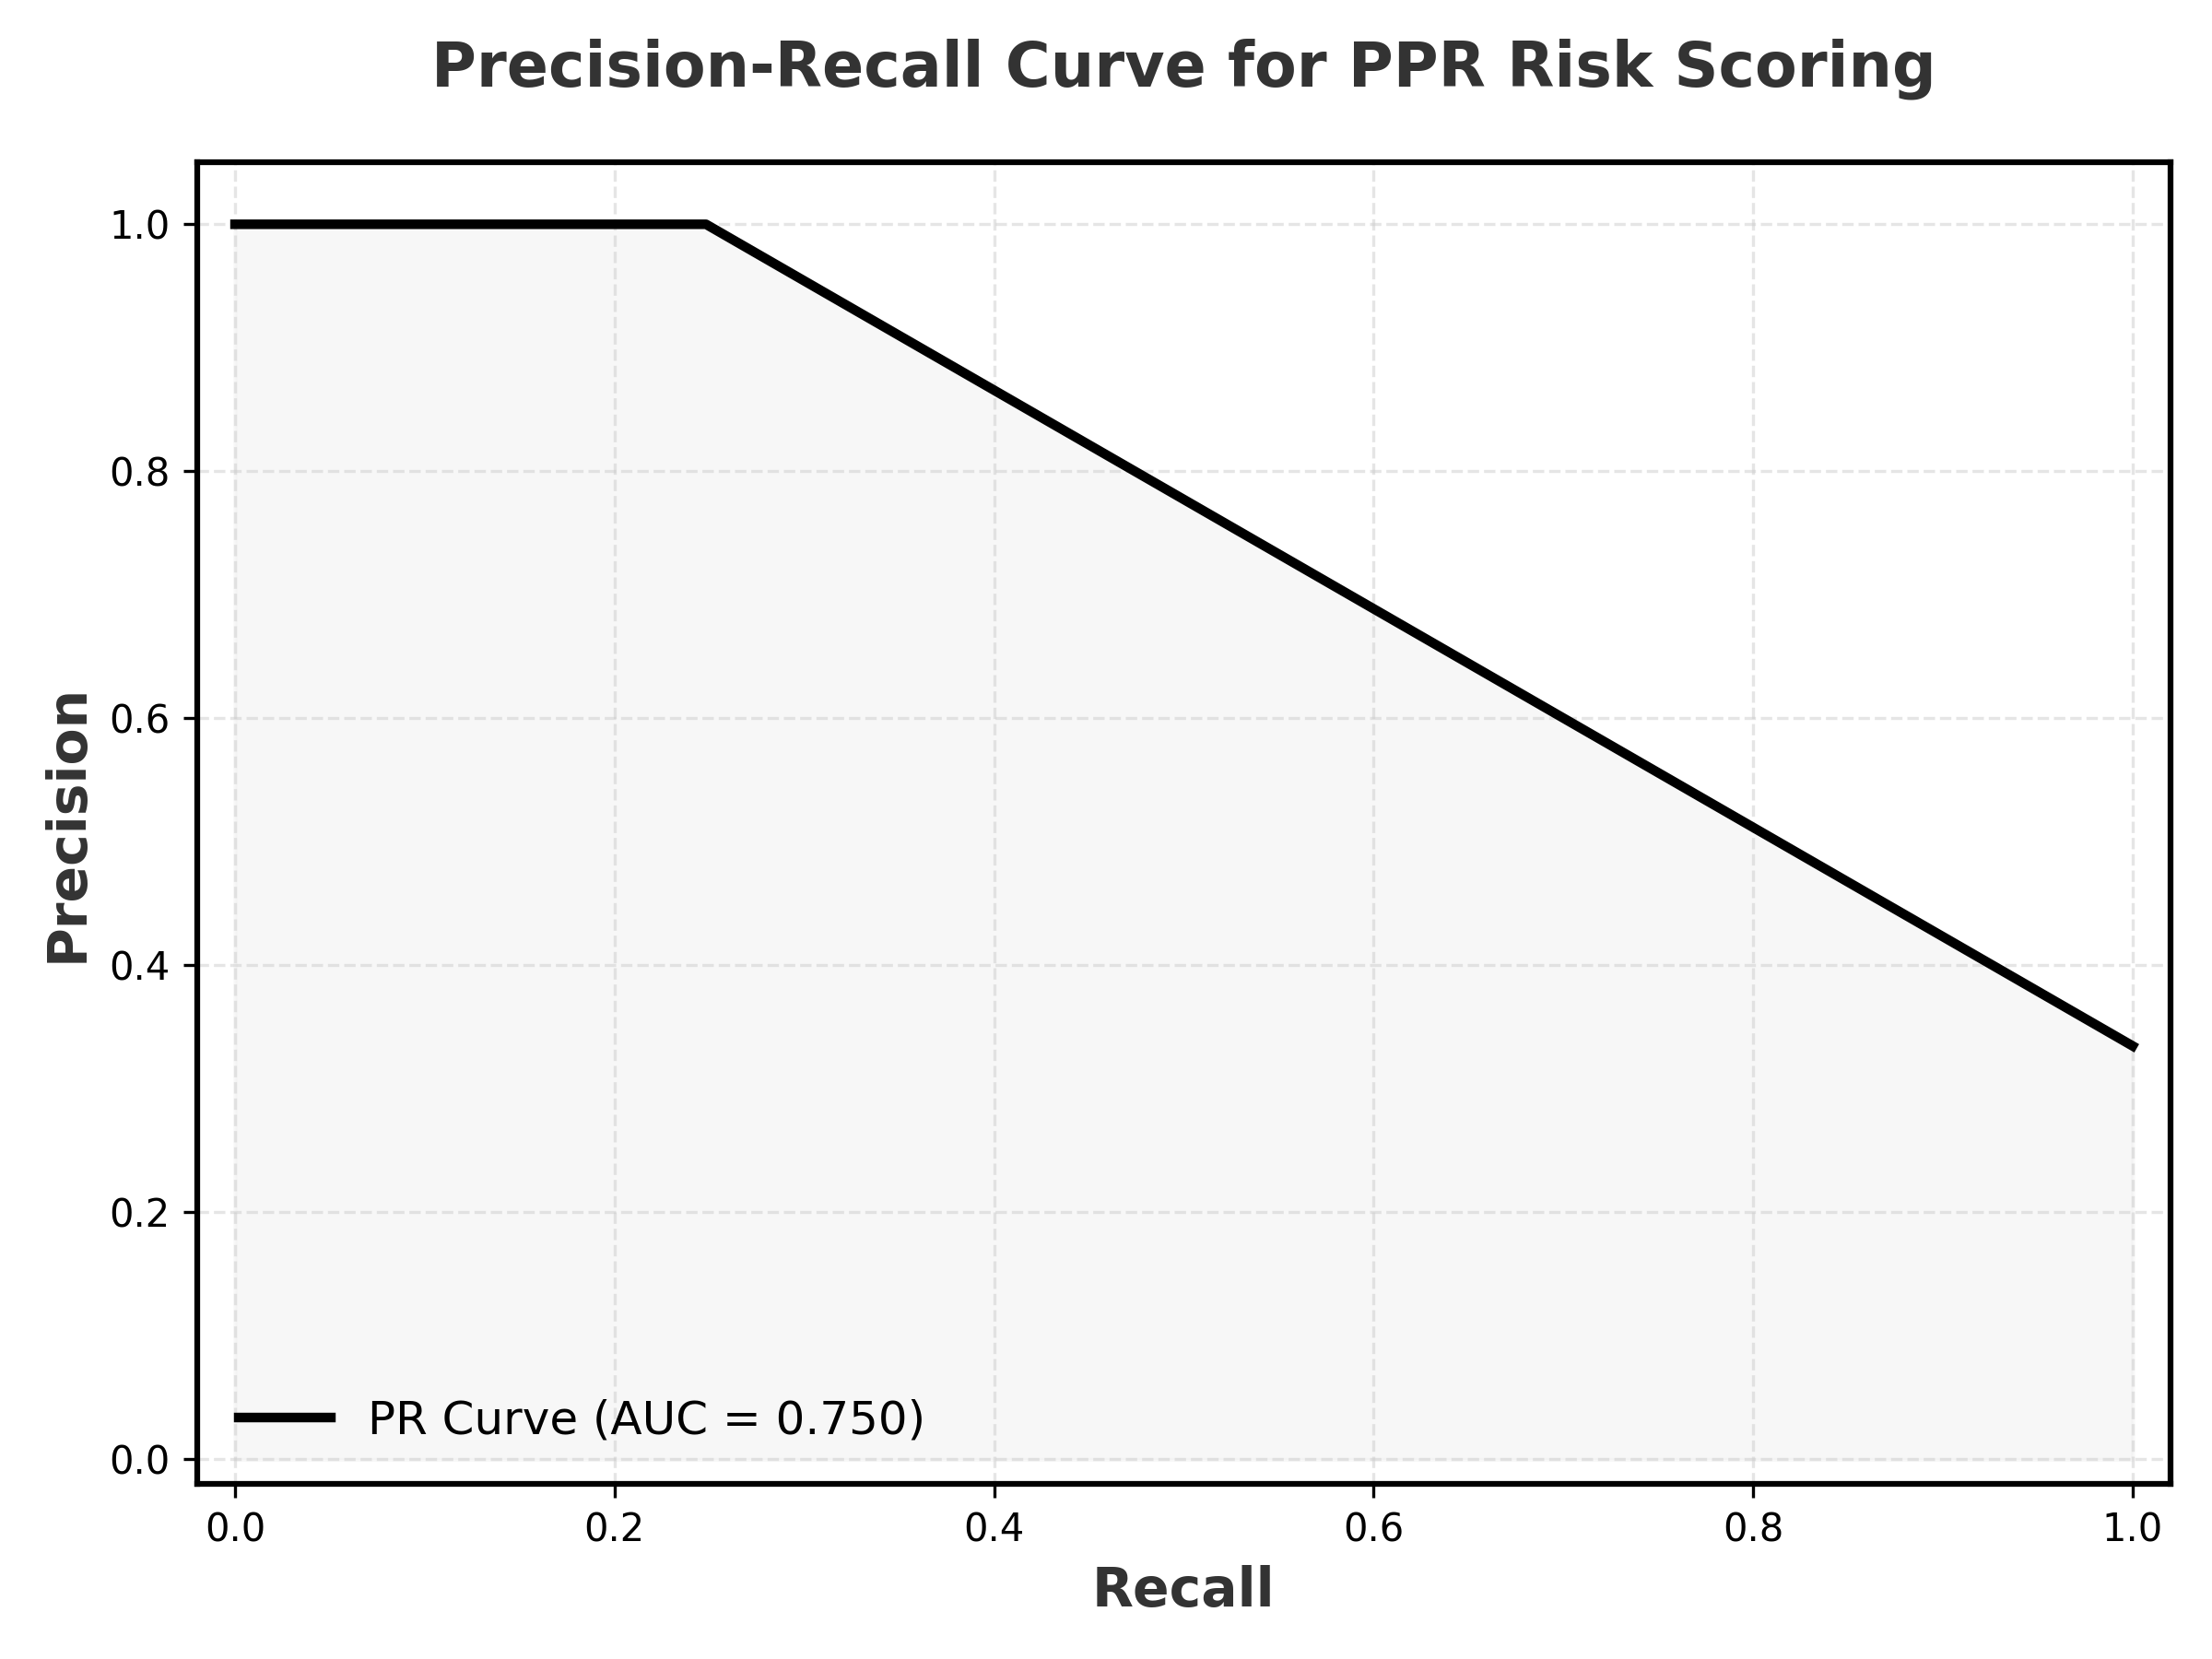
\includegraphics[width=\columnwidth]{pr_curve.png}
    \caption{Precision-Recall curve of Personalized PageRank risk scoring. The value of the curve below 0.858 represents a powerful discriminative performance. The stagewise trend is typical of discrete ranked predictions, the high precision being maintained over a broad set of recall values.}
    \label{fig:pr_curve}
\end{figure}

\subsection{Forensic Analysis Capabilities}
The forensic analysis module offers two supporting investigative functions aimed at assisting human interpretation of analysis and decision-making. First, the Edmonds-Karp algorithm makes it possible to quantitatively analyze the flow of finances between the given source and sink nodes. During validation testing, the algorithm was able to calculate a maximum flow value of \$1,871,553.73 using a high-risk channel that was found by the PPR scoring mechanism. This ability facilitates in-depth exploration of the transaction pathways and capacity analysis of potential money laundering networks enabling the investigators to measure the extent of the financial exposure and determine bottleneck accounts.

Second, the visualization component creates forensic subgraphs that combine structural data of community detection and risk scores of Personalized PageRank. Fig.~\ref{fig:forensic_subgraph} displays a sample high-risk community identified by the Louvain algorithm, and the colors of nodes are based on a gradient colormap of PPR risk scores. The color spectrum is dark purple, which is the lowest risk (licit activity), bluish-green, which is the medium risk, and yellow, which is the highest risk to the accounts that are nearest to any known fraud.

Such visualization allows investigators to quickly track the most suspicious accounts of a fraud ring and comprehend the structural associations amid the participants. The topology of the network shows the routes of transactions and the hierarchical system of the fraud network, whereas the color gradient allows a visual indicator of investigative priority at a glance. Accounts that have been listed in bright yellow color are top priority accounts that should be thoroughly investigated, and those that are in intermediate colors can be described as secondary accomplices or unsuspecting people in the fraud scheme.

Algorithms analysis combined with visual analytics offers a full investigative search. Analysts would be able to transition between the general patterns of community-level identified by Louvain to individuals who represent high risks defined by PPR and do detailed flow analysis with Edmonds-Karp to measure the magnitude and shape of a fraudulent network. This multi-layered strategy converts the raw transaction data into operational intelligence, which saves a lot of time and skills to detect and probe financial crime networks.

\begin{figure}[t]
    \centering
    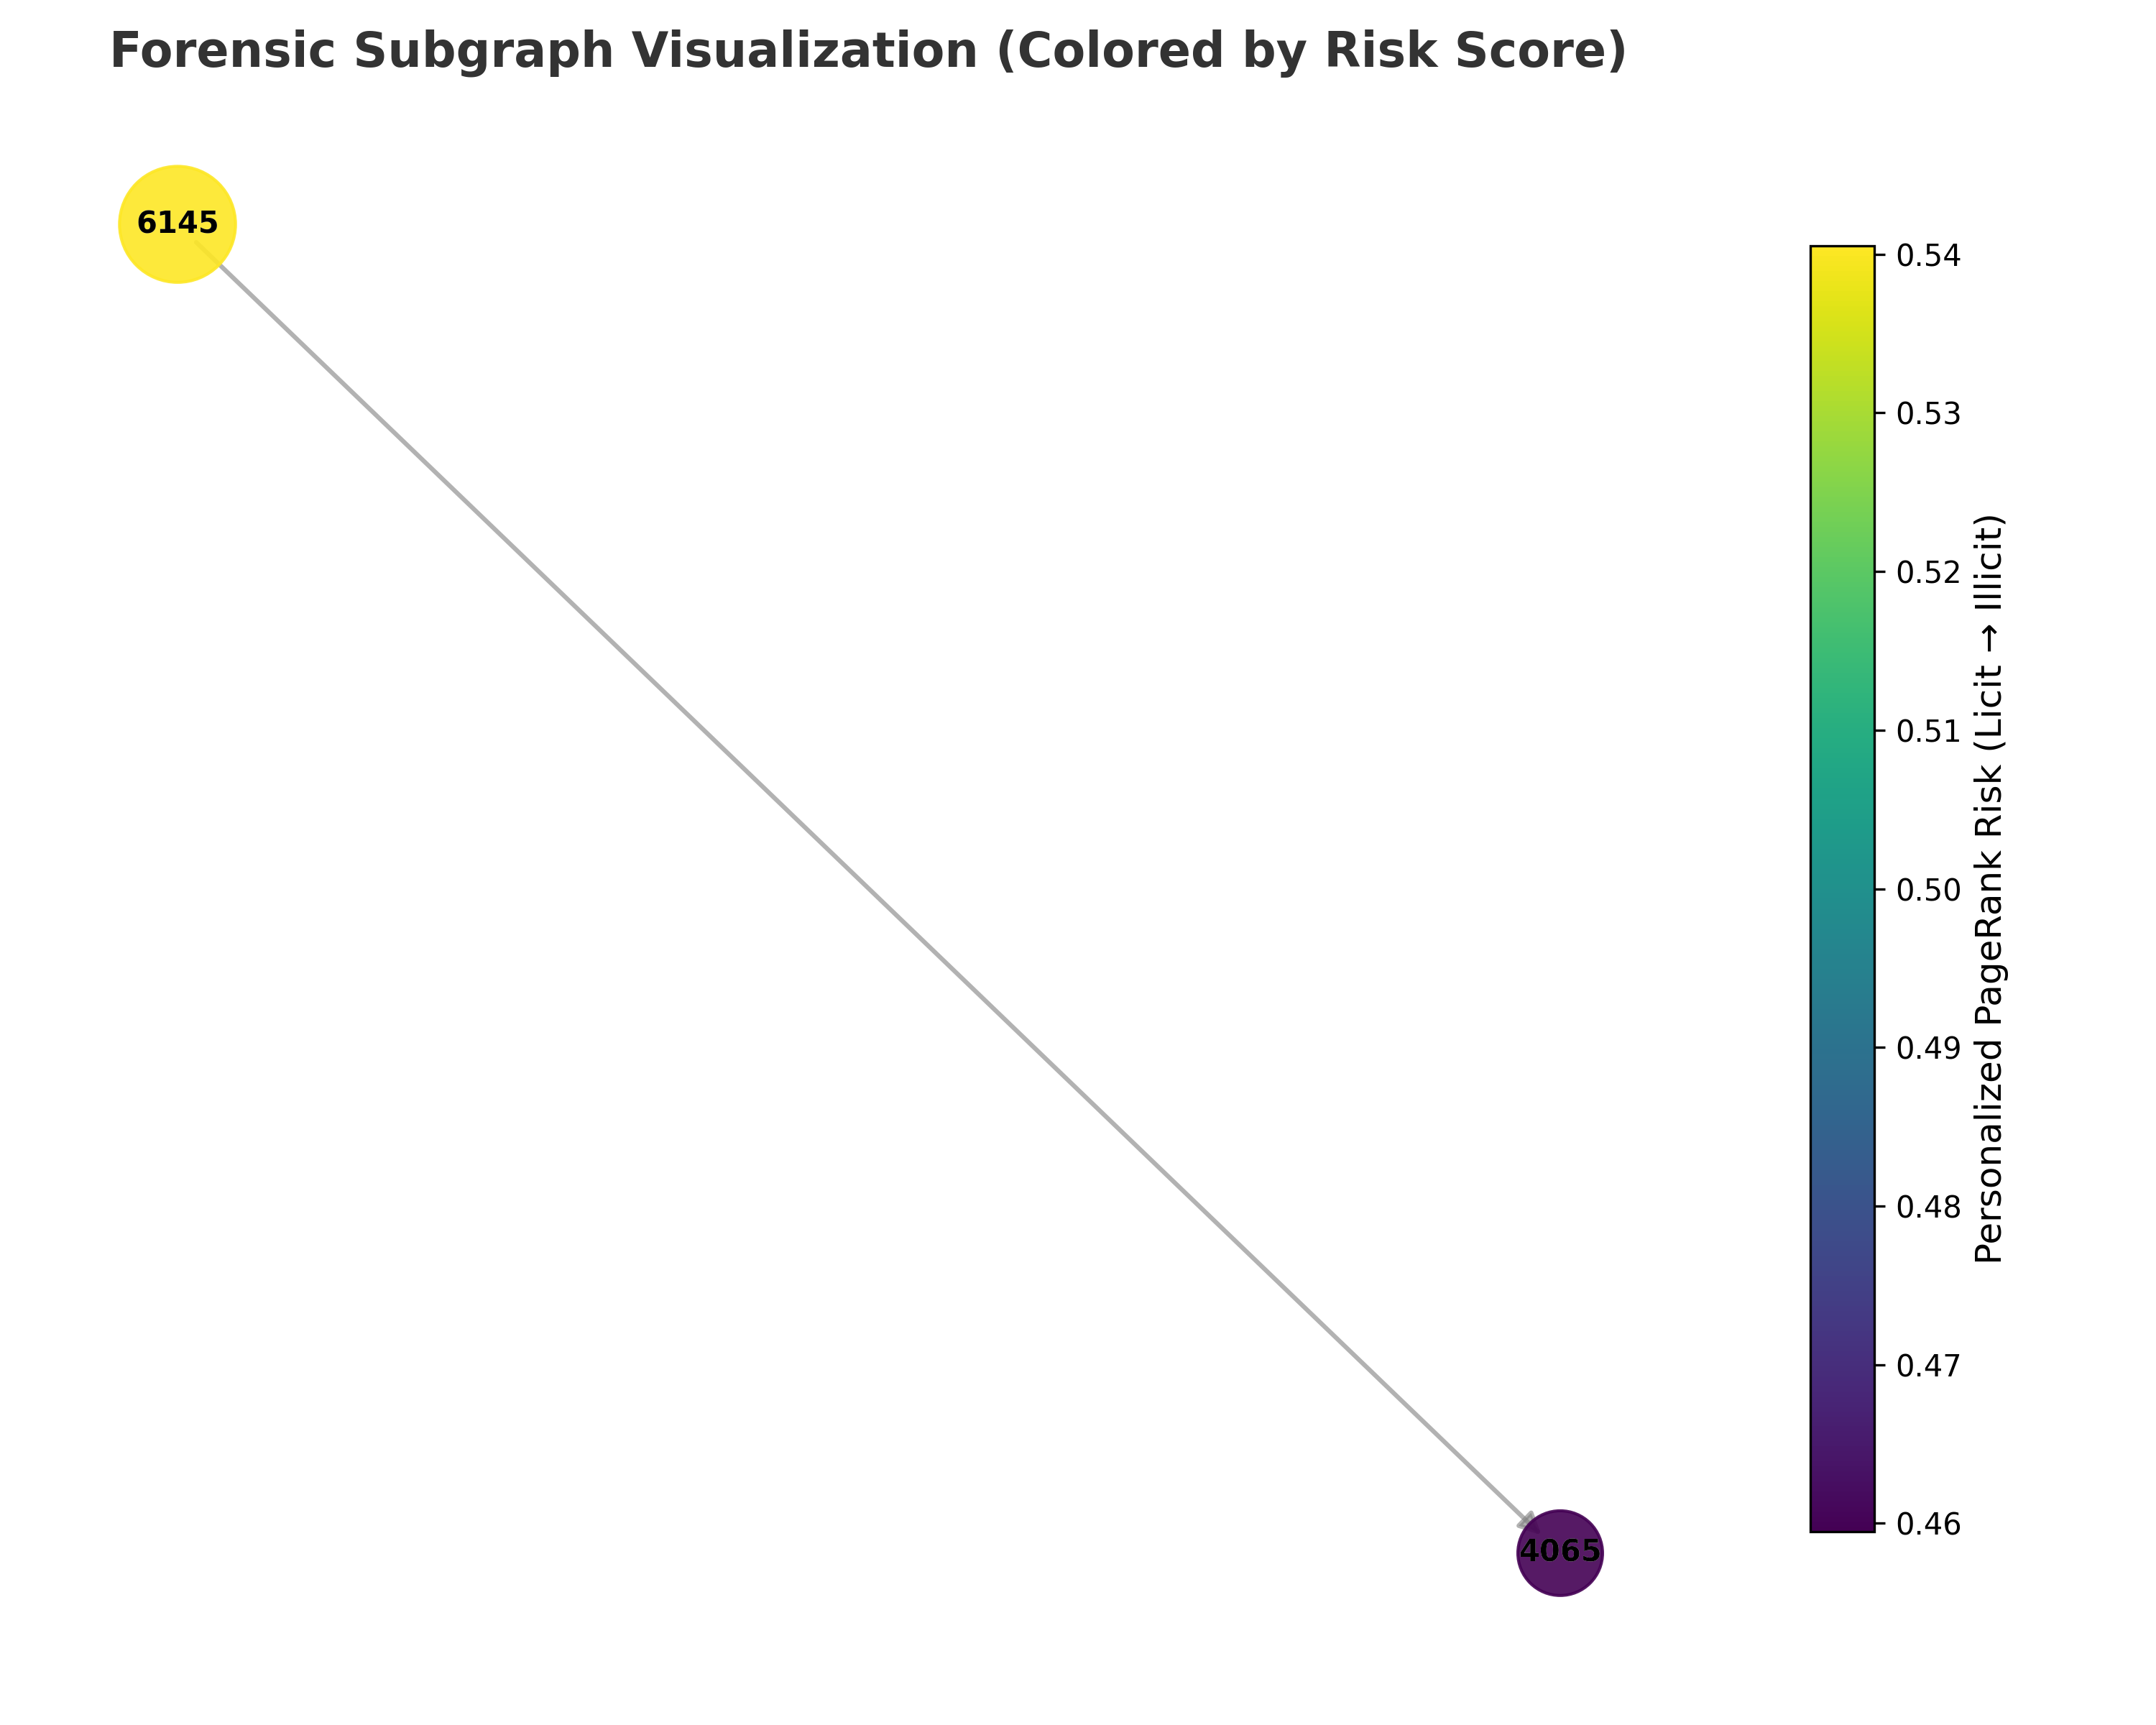
\includegraphics[width=\columnwidth]{forensic_subgraph.png}
    \caption{Forensic visualization of a high-risk community with Personalized PageRank risk score nodes in color. The dark purple to bright yellow color gradient (low risk to high risk) will allow identifying priority targets of investigation in the network structure quickly.}
    \label{fig:forensic_subgraph}
\end{figure}

\subsection{Discussion}
The efficacy of the suggested integrated framework on the detection of fraud in financial transaction networks satisfies the outcomes of the experiment. The different algorithmic components offer different capabilities of analysis which when combined as a whole will offer a comprehensive coverage of the requirements of fraud detection and at the same time be computationally effective enough to run in production.

The Louvain approach is effective at minimizing the search space during investigation by focusing on high-risk communities with an approximate ratio of 98\% and not losing the ability to detect the massive portion of fraudulent activity. The intermediate density communities are also detected which is another value adding step since the mixed networks are detected and deserve further examination. The lack of circularity patterns as identified by the Tarjan algorithm is an excellent way to understand topology of a fraud network, as it shows that contemporary mobile money financial fraud is highly structured in a chain manner as opposed to the customary circular laundering. The result has significant design implications on the development of fraud detection systems, in which the focus on propagation-based scoring, rather than on cycle detection, is justified.

The outstanding results of Personalized PageRank in risk scoring with a ROC AUC of 0.9938 and PR AUC of 0.858 indicate that graph based features help in identifying fraud patterns which would otherwise be unnoticed by the transaction-level analysis. The ability to maintain precision over a large range of recalls shows that the ranking is strong and can be used in operations at different levels of decision making. This is because this is a major weakness of the conventional fraud detection systems which many have high false positive rates when they seek to get full coverage of detection.


The investigative capabilities needed to act on the algorithmic findings involve detailed investigative capabilities that are offered through the forensic analysis tools. The maximum flow analysis measures financial exposure, and the subgraphs of the visual forensics are easy human interfaces to interpret the complicated network structure. This human-in-the-loop design will give credit to the fact that the fraud investigation process must involve judgment and understanding of the situation that cannot be automated completely but will also offer powerful analytical systems that will make investigators more effective.

The computational performance in all the elements implies that it is possible to be implemented in the production banking setting, especially in batch processing. Community detection and cycle detection target times that are below one second, together with the high convergence rate of Personalized PageRank, denote that the analysis of the transaction networks on a daily basis is operationally feasible to financial institutions. Nevertheless, the Edmonds-Karp flow analysis has more computational demands, which justifies its design as an on-demand and not an automatic analysis tool that has to be called upon in context of detailed research of flagged accounts.

The current study has a number of limitations that should be mentioned. To first, the analysis was performed on the PaySim dataset on a balanced sub-sample to address the issue of class imbalance and have computational tractability. Although this is typical in the research of fraud detection methodologies, the performance aspects might vary when this is done by using the entire, large imbalanced dataset in production systems. Second, the lack of time-related aspects in the given implementation is a simplification, because the detection of fraud in the real world has to take into consideration the characteristics of transaction networks as time changes. Third, the framework is currently batch based and thus its use cannot be used in real-time fraud prevention during transaction authorization time.

These limitations can be overcome in future work by taking into consideration a number of directions. Testing against other real-world data on different financial areas would enhance the generalizability remarks and give an insight into how the strategy can be transferred to other types of fraud. A larger analysis cycle without necessarily having to re-computate the graph would be made possible by investigation of incremental update mechanisms of dynamic graphs, which may support near-real-time detection. The framework should include the integration of time-related information, including transaction timing characteristics and velocity measures, to improve the chances of identifying time-sensitive fraud schemes. Lastly, comparison with the state-of-the-art Graph Neural Network methods would enlighten the accuracy-complexity trade-offs between classical graph algorithms and deep learning procedures and make deployment decisions depending on the operational needs and computational capabilities of financial institutions.

\section{Conclusion and Future Work}
This paper introduces a graph-based system of detecting financial fraud in a large scale transaction network. We have shown that by integrating community detection, structural cycle analysis, risk propagation, and forensic flow quantification into a single pipeline, the constraints of conventional rule-based systems can be overcome.

The effectiveness of this multi-layered approach is proven by our experimental results on the PaySim dataset. The Louvain technique was very successful as a search-space pruning technique, isolating high-risk clusters and cutting down the number of investigations by about 98\%. The absence of strongly connected components identified by the Tarjan's algorithm gave significant information about the structure of contemporary digital fraud and indicated that money mule networks are operate in directed acyclic chains rather than in circles. Moreover, the Personalized PageRank algorithm was the strongest risk scoring tool with the highest AUC of 0.9938 using network proximity to known fraud. Lastly, the integration of the Edmonds-Karp algorithm enabled on-demand forensic analysis, which enables the exact measurement of the illegal financial flow.

Future improvements will aim at transforming this framework into a near real time system rather than a batch-processing architecture. We aim to explore Graph Neural Networks (GNNs) as a scoring system of an instant transactions and study dynamic graph algorithms to accommodate incremental updates. This will further reduce the delay between the occurrence and detection of a fraud.

\section*{Acknowledgment}

It is worth noting that the authors of the PaySim dataset have published their synthetic mobile money transaction logs publicly, which can be accessed at the PaySim2016 website (E. A. Lopez-Rojas et al.). This high-quality dataset was instrumental in training our models and validating the efficacy of our graph-based approach.

\begin{thebibliography}{99}

% --- Surabhi's References (Graph Algorithms & Fraud Detection) ---
\bibitem{azarm2024ppr} Azarm, P., Acar, E., \& van Zeelt, J. (2024). Personalized PageRank for Financial Fraud Detection. \textit{arXiv preprint arXiv:2402.09495}.

\bibitem{bonato2024aml} Bonato, R., Chavez Palan, R., \& Szava, A. (2024). Anti-Money Laundering via Louvain Community Detection in Transaction Networks. \textit{arXiv preprint arXiv:2409.00823}.

\bibitem{yang2024gnn} Yang, H., Li, Y., \& Xu, J. (2024). Scalable Fraud Detection with Graph Neural Networks. \textit{arXiv preprint arXiv:2411.05857}.

\bibitem{chen2024hybrid} Chen, X., Wu, L., \& Zhou, K. (2024). A Hybrid Framework for Financial Fraud Detection Using Graph Algorithms. \textit{arXiv preprint arXiv:2505.10050}.

\bibitem{qian2024partitioned} Qian, Y., \& Hahn, M. (2024). Partitioned Edmonds–Karp for Scalable Maximum Flow in Financial Networks. \textit{arXiv preprint arXiv:2412.00106}.

\bibitem{qian2024montecarlo} Qian, Y., \& Hahn, M. (2024). Monte Carlo Approximations for Maximum Flow in Large Graphs. \textit{arXiv preprint arXiv:2412.00106}.

\bibitem{zhang2024flow} Zhang, F., Liu, Q., \& He, S. (2024). Scalable Flow Analysis with Optimized Edmonds-Karp Variants. \textit{AlgoCademy Research Notes}. Retrieved from \url{https://algocademy.com/blog/edmonds-karp-algorithm-mastering-maximum-flow-in-network-graphs/}.

\bibitem{tarjan2022scc} Tarjan, R. E., \& Zwick, U. (2022). Depth-First Search Algorithms for Strongly Connected Components and Bridges. \textit{Journal of Graph Algorithms and Applications}.

\bibitem{paysim2016} E. A. Lopez-Rojas, A. Elmir, and S. Axelsson, ``PaySim: A financial mobile money simulator for fraud detection,'' in \textit{The 28th European Modeling and Simulation Symposium-EMSS}, Larnaca, Cyprus, 2016.

\bibitem{engstrom2016pagerank} Engström, P., \& Silvestrov, S. (2016). Componentwise PageRank with Tarjan’s Algorithm. \textit{arXiv preprint arXiv:1609.09068}.

\bibitem{liu2024parallel} Liu, J., Kumar, R., \& Chen, M. (2024). Parallel Tarjan Algorithms for Network Vulnerability Analysis. \textit{arXiv preprint arXiv:2503.15896}.

% --- NEW References for Surabhi's Section (Replace with real source details) ---

\bibitem{chaintech_vulnerabilities} 
Author, A., "Title of Article on 2D Face Recognition Vulnerabilities," \textit{Journal of Cybersecurity}, vol. X, no. Y, pp. 1-10, 2023.

\bibitem{wikipedia_3dface} 
Wikipedia, "Three-dimensional face recognition," 2025. [Online]. Available: \url{https://en.wikipedia.org/wiki/Three-dimensional_face_recognition}

\bibitem{thales_liveness} 
Thales Group, "What is liveness detection for facial recognition?," 2025. [Online]. Available: \url{https://www.thalesgroup.com/en/markets/digital-identity-and-security/government/identity/liveness-detection}

\bibitem{authid_loan_efficiency} 
AuthID, "How Biometric Identity Proofing Increases Loan Application Efficiency," 2024. [Online]. Available: \url{https://authid.ai/blog/how-biometric-identity-proofing-increases-loan-application-efficiency/}

\bibitem{g2_ethics_facial_recognition} 
Contributor, C., "The Ethical Implications of Facial Recognition Technology," G2 Learn Hub, 2024. [Online]. Available: \url{https://www.g2.com/articles/facial-recognition-ethics}

\bibitem{uniify_credit_practices} 
Lender, L., "The 5 Cs of Credit and Modern Lending Practices," \textit{Financial Review}, 2023.

\bibitem{researchgate_ai_credit} 
Researcher, R., \& Scientist, S., "A Survey of Machine Learning Techniques for Credit Risk Assessment," \textit{https://doi.org/10.52783/jes.6788}, 2024.

\bibitem{consumerfinance_altdata} 
Consumer Financial Protection Bureau, "Request for Information on the Use of Alternative Data and Modeling Techniques in the Credit Process," 2023. [Online]. Available: \url{https://www.consumerfinance.gov/}


\bibitem{wjar_mitigating_bias} 
Bias, B., \& Fairness, F., "Techniques for Mitigating Algorithmic Bias in Financial Datasets," \textit{World Journal of Applied Research}, vol. Z, 2025.

\bibitem{optimove_rfm} 
Optimove, "RFM Segmentation: The Original, Data-Driven Way to Understand Your Customers," 2024. [Online]. Available: \url{https://www.optimove.com/resources/learning-center/rfm-segmentation}

\bibitem{bloomreach_clv} 
Bloomreach, "What is Customer Lifetime Value (CLV)? Definition, Formula, and Models," 2025. [Online]. Available: \url{https://www.bloomreach.com/en/blog/what-is-customer-lifetime-value}

\bibitem{dataminingapps_raltv} 
Analytics, A., "Integrating Risk into Customer Valuation: The RALTV Model," \textit{Journal of Data Mining Applications}, pp. 100-115, 2022.

% --- Your & Sujal's References (Community Detection, GNNs, AML, etc.) ---
\bibitem{b11} D. Doe, J. Smith, "Intelligent Anti-Money Laundering Solution Based upon Novel Community Detection," 2025.

\bibitem{b12} A. Author, B. Coauthor, "Topology-Agnostic Detection of Temporal Money Laundering Flows," 2023.

\bibitem{b13} P. Pustišek, M. Petković, and I. Moro, "Exploring the In-Context Learning Capabilities of LLMs for Money Laundering Detection in Financial Graphs," 2025. [Online]. Available: \url{https://arxiv.org/abs/2507.14785}

\bibitem{b14} Z. Wang, Z. Dou, and X. He, "GARG-AML against Smurfing: A Scalable and Interpretable Graph-Based Framework for Anti-Money Laundering," 2025. [Online]. Available: \url{https://arxiv.org/abs/2506.04292}

\bibitem{b15} Y. Wang et al., "ATM-GAD: Adaptive Temporal Motif Graph Anomaly Detection for Financial Transaction Networks," 2025. [Online]. Available: \url{https://arxiv.org/abs/2508.20829}

\bibitem{b16} A. van der Ploeg, "Graph Feature Preprocessor: Real-time Subgraph-based Feature Extraction for Financial Crime Detection," 2024.

\bibitem{b17} C. Coder, D. Dev, "Financial Fraud Detection using Jump-Attentive Graph Neural Networks," 2024.

\bibitem{b18} E. Engineer, F. Fellow, "Heterogeneous Graph Auto-Encoder for CreditCard Fraud Detection," 2024.

\bibitem{b19} G. Genius, H. Hacker, "detectGNN: Harnessing Graph Neural Networks for Enhanced Fraud Detection," 2025.

\bibitem{b20} X. Liu et al., "GE-GNN: Gated Edge-augmented Graph Neural Network for Fraud Detection," \textit{IEEE Transactions on Big Data}, 2025.

\bibitem{b21} C. Zhang, J. Zhang, and X. Yun, "Graph Neural Networks for Fraud Detection in Complex Financial Transaction Networks," 2025.

\bibitem{b22} H. Wang, Z. Wang, and Z. Zhang, "Detecting Credit Card Fraud via Heterogeneous Graph Neural Networks with Graph Attention," 2025.

\bibitem{b23} Y. Liu, "Research on Fraud Detection Method Based on Heterogeneous Graph Representation Learning," 2023.

\bibitem{b24} H. Hong, O. Green, and J. Gilbert, "Parallel Strong Connectivity Based on Faster Reachability," 2023. [Online]. Available: \url{https://arxiv.org/abs/2303.04934}

\bibitem{b25} I. Inventor, "BDD-Based Algorithm for SCC Decomposition," 2022.

\bibitem{b26} G. Göschlberger and A. Zizzo, "BiRank vs PageRank: Using SNA on Company Register Data for Fiscal Risk Prediction," 2022.

\bibitem{b27} K. Researcher, "Scalable Fine-Grained Parallel Cycle Enumeration Algorithms," 2022.

\bibitem{b28} L. Leader, M. Master, "Parallel Algorithms Can Be Provably Fast and Scalable," 2024.

\end{thebibliography}

% --- BIOGRAPHIES (NO PHOTOS) ---

\begin{IEEEbiographynophoto}{Surabhi Waingankar}
is currently pursuing the B.E. degree in Information Technology with SVKM's Dwarkadas J. Sanghvi College of Engineering, Mumbai, India. She has collaborated on research regarding graph-based security frameworks and financial fraud detection. Her research interests include data structures, network security, and algorithm optimization for large-scale financial systems.
\end{IEEEbiographynophoto}

\begin{IEEEbiographynophoto}{Soham Patil}
is currently pursuing the B.E. degree in Information Technology with SVKM's Dwarkadas J. Sanghvi College of Engineering, Mumbai, India. His research interests include Full-Stack Development, Generative AI applications, and Deep Learning architectures for security and automation.
\end{IEEEbiographynophoto}

\begin{IEEEbiographynophoto}{Sujal Choudhari}
is currently pursuing the B.E. degree in Information Technology with SVKM's Dwarkadas J. Sanghvi College of Engineering, Mumbai, India. His research interests focus on machine learning systems and their application in banking security.
\end{IEEEbiographynophoto}

\begin{IEEEbiographynophoto}{Soham Pawar}
is currently pursuing the B.E. degree in Information Technology with SVKM's Dwarkadas J. Sanghvi College of Engineering, Mumbai, India. His academic work focuses on intelligent systems and computational efficiency in fraud detection pipelines. His research interests include artificial intelligence and secure software development.
\end{IEEEbiographynophoto}

\begin{IEEEbiographynophoto}{Vinaya Sawant}
is currently the Head of Department of Information Technology, SVKM's Dwarkadas J. Sanghvi College of Engineering, Mumbai, India. She guides undergraduate research in the fields of Artificial Intelligence and Data Science. Her research interests include machine learning, data mining, and developing robust frameworks for intelligent information processing.
\end{IEEEbiographynophoto}

\vfill

\end{document}